\documentclass{article}
\usepackage[margin=3cm]{geometry}
\usepackage{tikz}
\usepackage{float}
\usepackage{caption}
%\setlength\textwidth{6.875in}
%\setlength\textheight{8.875in}
% set both margins to 2.5 pc
%\setlength{\oddsidemargin}{-0.1875in}% 1 - (8.5 - 6.875)/2
%\setlength{\evensidemargin}{-0.1875in}
%\setlength{\marginparwidth}{0pc}
%\setlength{\marginparsep}{0pc}%
%\setlength{\topmargin}{0in} \setlength{\headheight}{0pt}
\setlength{\headsep}{0pt}
\setlength{\footskip}{37pt}%
%\setlength{\columnsep}{0.3125in}
%\setlength{\columnwidth}{3.28125in}% (6.875 - 0.3125)/2 = 3.28125in
%\setlength{\parindent}{1pc}
%\newcommand{\myMargin}{1.00in}
%\usepackage[top=\myMargin, left=\myMargin, right=\myMargin, bottom=\myMargin, nohead]{geometry}
\usepackage{epsfig,graphicx}
\usepackage{palatino}
\usepackage{fancybox}
\usepackage{hyperref}
\usepackage{url}
\usepackage{ctex}
\usepackage[procnames]{listings}
\usepackage{multicol}
\usepackage{pdfpages}
\usepackage{calc}

\lstdefinelanguage{scala}{
	morekeywords={abstract,case,catch,class,def,%
		do,else,extends,false,final,finally,%
		for,if,implicit,import,match,mixin,%
		new,null,object,override,package,%
		private,protected,requires,return,sealed,%
		super,this,throw,trait,true,try,%
		type,val,var,while,with,yield},
	sensitive=true,
	morecomment=[l]{//},
	morecomment=[n]{/*}{*/},
	morestring=[b]",
	morestring=[b]',
	morestring=[b]"""
}

\usepackage{color}
\definecolor{dkgreen}{rgb}{0,0.6,0}
\definecolor{gray}{rgb}{0.5,0.5,0.5}
\definecolor{mauve}{rgb}{0.58,0,0.82}

% Default settings for code listings
\lstset{frame=tb,
	language=scala,
	aboveskip=3mm,
	belowskip=3mm,
	showstringspaces=false,
	columns=fixed, % basewidth=\mybasewidth,
	basicstyle={\small\ttfamily},
	numbers=none,
	numberstyle=\footnotesize\color{gray},
	% identifierstyle=\color{red},
	keywordstyle=\color{blue},
	commentstyle=\color{dkgreen},
	stringstyle=\color{mauve},
	frame=single,
	breaklines=true,
	breakatwhitespace=true,
	procnamekeys={def, val, var, class, trait, object, extends},
	procnamestyle=\ttfamily\color{red},
	tabsize=2
}

\lstnewenvironment{scala}[1][]
{\lstset{language=scala,#1}}
{}
\lstnewenvironment{cpp}[1][]
{\lstset{language=C++,#1}}
{}
\lstnewenvironment{bash}[1][]
{\lstset{language=bash,#1}}
{}
\lstnewenvironment{verilog}[1][]
{\lstset{language=verilog,#1}}
{}

\lstset{frame=, basicstyle={\footnotesize\ttfamily}}
\newcommand{\chinesedash}{\rule[.7ex]{\widthof{二字}}{0.5pt}}
\newcommand{\todo}[1]{\emph{TODO: #1}}
\newcommand{\comment}[1]{\emph{Comment: #1}}

% uncomment following for final submission
\renewcommand{\todo}[1]{}
\renewcommand{\comment}[1]{}

\newenvironment{commentary}
{ \vspace{-0.1in}
  \begin{quotation}
  \noindent
  \small \em
  \rule{\linewidth}{1pt}\\
}
{
  \end{quotation}
}

\title{多发射乱序CPU的RTL级实现与验证}
\author{ 开题报告\\
{周盈坤} \\
{\tt  zhouyingkun15@mails.ucas.ac.cn}}
\date{\today}

\newenvironment{example}{\VerbatimEnvironment\begin{footnotesize}\begin{Verbatim}}{\end{Verbatim}\end{footnotesize}}
\newcommand{\kode}[1]{\begin{footnotesize}{\tt #1}\end{footnotesize}}

\def\code#1{{\tt #1}}
\newcommand{\myFrame}[2]{\tikz[overlay, remember picture] \draw ([xshift=2.8cm,yshift=-#1cm]current page.north west) rectangle ([xshift=-2.8cm,yshift=#2cm]current page.south east);}
\def\note#1{\noindent{\bf [Note: #1]}}
%\def\note#1{}

%\usepackage{biblatex}
%\addbibresource{reference.bib}

\begin{document}
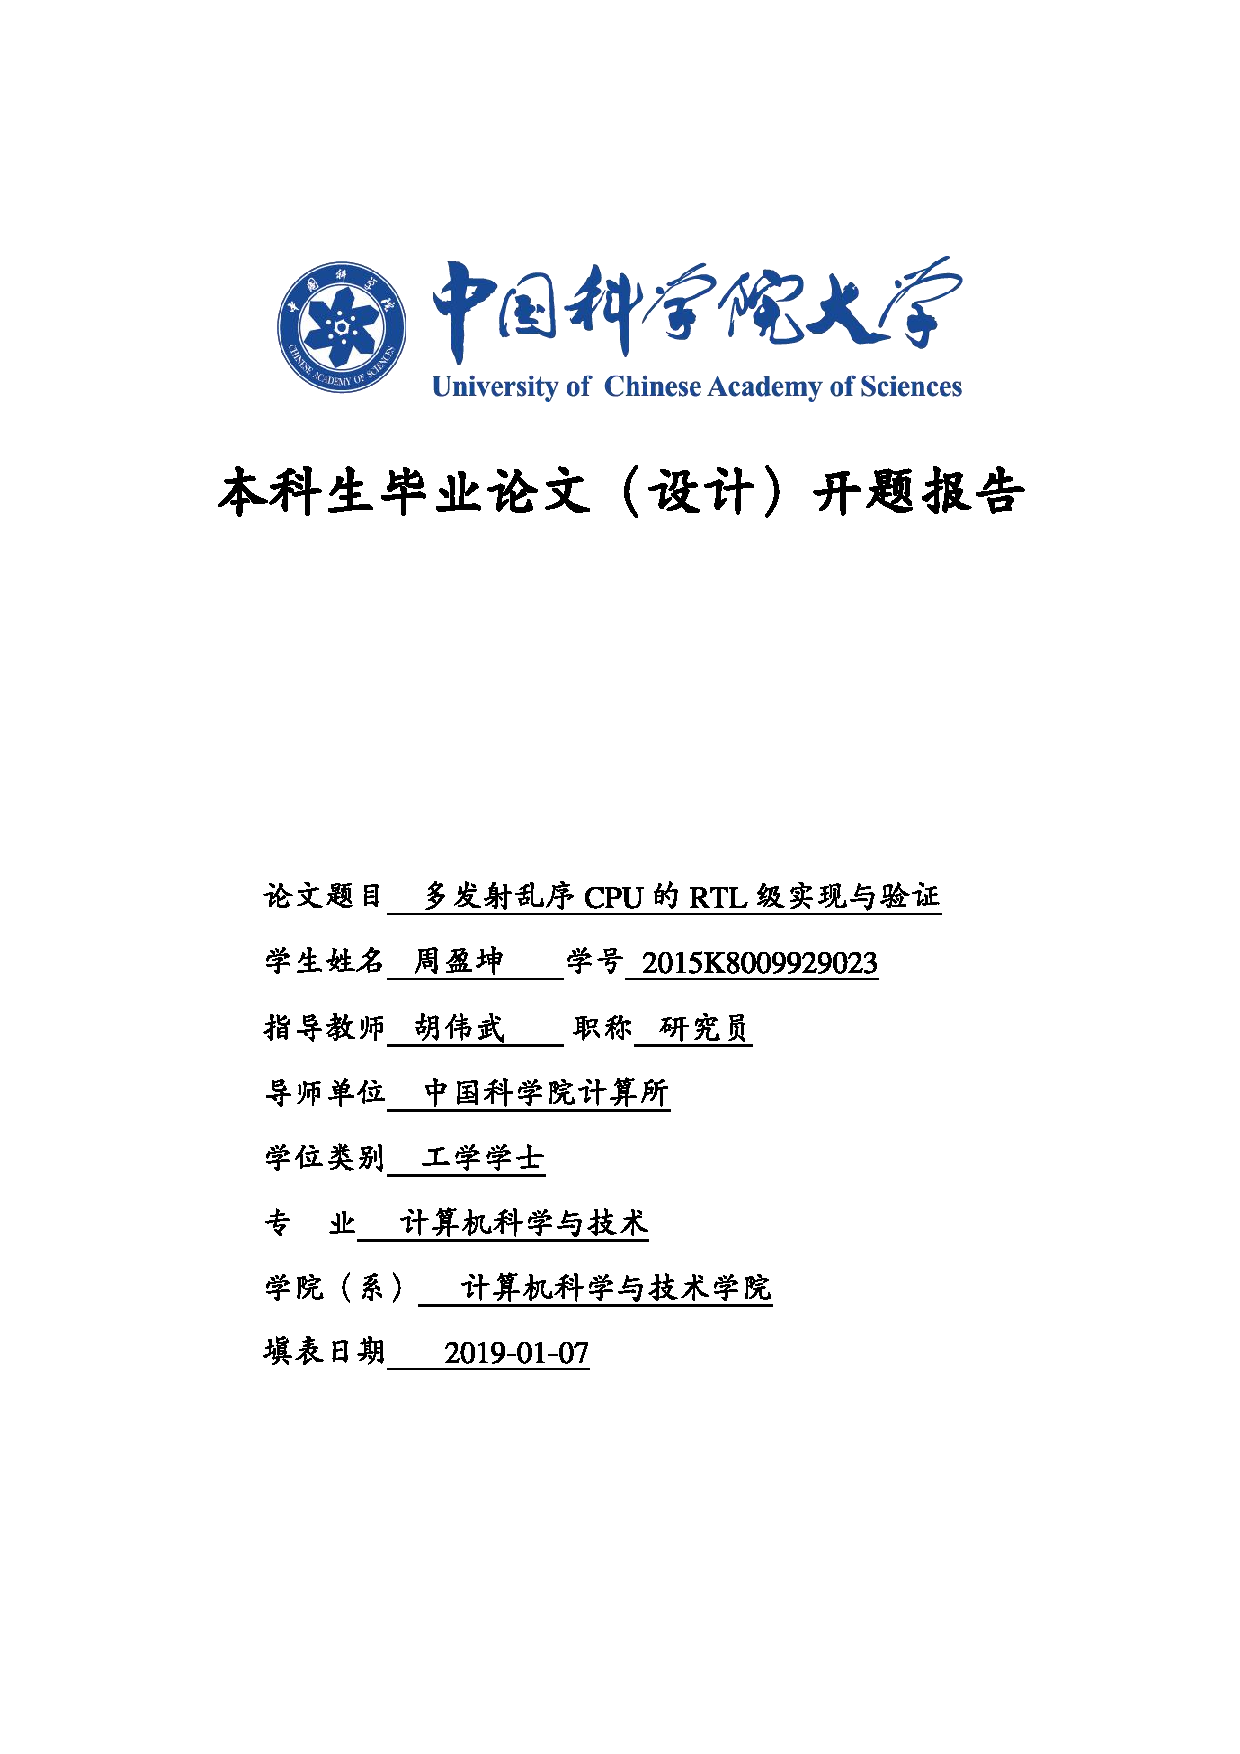
\includepdf[pages={1,2,3},scale=1.1]{kaiti.pdf}
\includepdf[pages=4,scale=1.15,offset=0mm -10mm]{kaiti.pdf}
%\maketitle{}
% \myFrame{3}{3}
% \begin{figure}[!hb]
% 	\vspace{-0.9cm}
% 	\hspace{-0.55cm}
% 	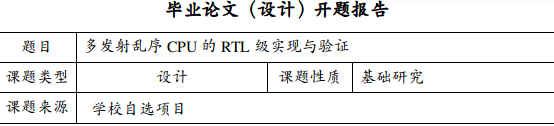
\includegraphics[width=16.5cm,height=4cm]{title.png}
% \end{figure}

% \section*{选题的背景及意义:}
% \begin{commentary}
% 	计算机领域,体系结构者扮演的是上帝的角色。上帝造万物、制规律,但却察觉不到。用户不会关心在程序的背后何种指令是按照何种方式被执行,只会在乎在计算机世界里跑的应用程序如否满足自己的需求,是否流畅。

% 	操作体统犹如国王,国王管理着国家。国王即天子,和上帝ISA紧紧绑定。当今世界的三大国家的国王为Windows, MacOS, Linux. 国王有着极大的威严,号令着所有在这个国家的领域上运行的程序。如果需要时不时跨国,便可体会到不同国度的差异。

% 	普通软件程序犹如国家的臣民和机构,它们必须遵从国家的规章制度,服从国王调度,涉及到关键资源的操作,必须上报国家,由国家安排与分配,跨国公司也概莫能外。

% 	编译器则是使者,无论是王公贵族还是黎明百姓,都需要经由它来与上帝沟通,使之从高级语言转化为机器码。
% \end{commentary}
% 体系结构迎来了开源之光,这是一个大的背景。RISC-V开源的项目越来越多,有微处理器设计的如Rocket和BOOM;有更高级的刻画电路的语言的如Chisel;也有针对RISC-V的调试工具如Spike,以及上层已经移植好的基础软件栈如Linux,GCC和LLVM。大大降低了独立设计出一款高性能处理器以及在上面跑系统的难度与门槛。所以计划本科毕业设计顺着这股大的潮流先基于64位RISC-V自行实现一款高性能的处理器。同时编写调试的过程也是在学习开源资料中优秀的思想的过程,也是不断提高自我修养的过程。事成之后再移植到MIPS的ISA上,就可以做到同样架构对比两个ISA之间的优劣势了,这样更加客观。

% 但是本科阶段没有发论文的打算,一是体系结构这个领域十年磨一剑,仅凭本科毕设估计很难有成色;二是在本科阶段参与和体系结构、操作系统、编译原理有关的基础性工作,打好以后研究的基础,所以借设计一款高性能的CPU并能够运行系统来提高自己软硬件的素养就是这个选题的意义所在。

%曾与张科老师的交流中他问过像这样的毕设工作有什么意义,我倒觉得讲求实用性应该是建立在不断完善自己的学术工程素养基础之上的。也曾与汪文祥老师沟通过,他提出首先这个毕设的题目是偏重于工程实现的,论文方面不一定出彩;其次工作量大,不一定能够完成。所以要做好心理准备并一步步脚踏实地去完成毕设的工作。

% \newpage
\myFrame{3}{3}
\section*{国内外本学科领域的发展现状与趋势:}\label{state}

\section{语言与表示}
\subsection{Verilog}
Verilog是目前流行通用的硬件描述语言,表现能力强,语言设计参考的是C语言而且最开始设计出来是用作仿真的,因而有很多用于仿真的语法。但是真正可以用于综合电路的语言并不多,比较常规的有组合逻辑的assign语句,时序逻辑的时钟上升沿触发的同步电路逻辑\newline always@(posedge clk) begin ... end. 辅以generate的写法,避免相同的逻辑代码重复冗余。
\subsection{Scala}
Scala是一门非常有野心的语言。它并不是从头开始构建的语言,而是依附在JAVA的平台之上,能够复用JAVA已有的library。这本身就是一个很好的考虑。甚至可以说Scala就是扩展在JAVA之上的脚本语言。它同时兼顾面向对象与函数化编程,并且它还是静态类型的语言,所以不同于python。而做到脚本语言的同时可以使静态类型编译的关键一点就是类型编译时推导,只需要在关键的地方声明类型即可,比如函数或者方法定义时的传入参数列表。

Verilog和Scala,风牛马不相及。然后从本质上来看,所有的语言都服务于一个目的\chinesedash 描述逻辑。而现在这个需求更加的具体化,那就是描述电路的逻辑。所以再往下思考,电路的逻辑需要什么语言要素来刻画。
\begin{enumerate}
	\item 模块化。功能电路的设计,CPU的设计是模块化的。
	\item 函数化。功能电路关注点在于输入input,输出ouput,这一点和函数很像。
\end{enumerate}
分析得出这两个特征,会发现Scala的面向对象和函数化编程是多么契合电路的逻辑设计。如此一来Scala就有描述电路的可能。除了支持的语言特性吻合电路设计的需求外,Scala作为一种强类型的语言,同样是电路刻画需要的(Verilog也可以看做是强类型的)。而且Scala是脚本语言,同样有优势,首先脚本语言简洁,其次电路的描述并没有很大的计算量,这恰恰就是脚本语言所擅长的。

为了代码的简洁与复用,语言的高级化是在所难免的。通用的编程语言从C到C++再到Java再到如今的pyhton。然而硬件的描述语言却一直停留在最初的Verilog,究其原因,电路描述高级语言化的障碍有两点:
\begin{enumerate}
	\item 时序逻辑高级语言应该如何描述?
	\item 随着语言的高级化,会不会使得电路的编写模糊化,使得所写的电路很难对应到实际的物理电路上,就像高级语言对垃圾回收做了透明化一样。这恰恰是硬件的工程师所不愿意看到的,因为电路设计要了解电路的所有实现细节。
\end{enumerate}

\subsection{chisel}
世上无难事,只怕有心人。Chisel的出现,将Verilog和Scala连接起来,将上述的可能变为了现实。那么Chisel是如何(初步)打消上述的两个障碍和顾虑的呢?那就要看Chisel是怎么进行抽象的。
\begin{enumerate}
	\item 组合电路的对应于Verilog中的wire,赋值用assign语句,也可以直接在定义的时候赋值。而Chisel首先用的就是两类的数据类型来描述,分别是UInt和Bool。Bool只是为了强调变量是1 bit的代表真假的布尔逻辑变量。而wire类型变量的赋值有两种形式
	\begin{itemize}
		\item 初始定义的 \textbf{=} 运算符 
		\begin{scala} 
			val pc = UInt() 
		\end{scala}
		
		如上并不是真正的赋值,而是类型的申明,而且如果wire的 width省略,Chisel会在编译的时候自动在以后的真正赋值中推导出来。
		\item 因为val在Scala中是不可变量,也就是变量名指针所指的对象不能更改,所以chisel中引入\textbf{:=}运算符(本质上Scala将其抽象为对象的方法,这是一个非常高明的抽象)来进行重赋值。
		\begin{scala} 
			pc := pcReg + 4.U 
		\end{scala}
		
		这个时候Chisel编译器就可以从right hand side表达式中推导出pc的宽度。~\cite{chisel}
		
	\end{itemize}
	\item 时序电路对应于Verilog中的reg,赋值需要用到always语句。而在Chisel对其进行了一段抽象,首先它没有具体的类型,是一个Reg的元器件。其次这个元器件有两面\chinesedash input和output。而output可以理解为input信号延迟一拍的副本。所以严格来讲,Reg是有类型的,就是input端所连的变量的类型,在reg类型变量的定义中还可以指明reset的初始值。如下例:
	\begin{scala}
		val pcReg = Reg(next = pcNext, init = 0.U(32.W))
	\end{scala}
	在当前的版本的Chisel中,时钟和复位是全局信号,是隐式申明的。~\cite{chisel}
	\item := 运算符将右手表达式代表的组合逻辑连线到左手变量代表的目的节点上。如果涉及到寄存器,用变量x来表示,那么x若出现在右手边,用到的就是output端;如果出现在左手边,用的就是input端。~\cite{chisel}
	\item 对于wire类型和reg类型的变量,Chisel统一抽象为了node。所以整个电路图就是由node组成的图。具体来讲,如果是纯组合逻辑,那么这个图就是有向无环图,所以Chisel是可以对于设计中出现的组合环进行报错,从而规避了仿真中出现的奇怪的现象。唯一存在有环的情况是时序电路。而且依据这个图,可以用verilator工具生成高速的C++的simulator~\cite{chisel}。
	\item 有了基础的抽象,Chisel可以在其上利用面向对象的方法和继承的手法构建更为大型,更为抽象的数据结构,比如memory。
	\item 同时,在Verilog对于模块的刻画用了module的写法,而在Chisel中则是用户自定义class来extends 叫做Module的super class来刻画电路模块,并且对于port接口,定义了一个IO的类。如下例~\cite{chisel}:
	\begin{scala}
	class Mux2 extends Module {
		val io = IO(new Bundle{
			val sel = Input(UInt(1.W))
			val in0 = Input(UInt(1.W))
			val in1 = Input(UInt(1.W))
			val out = Output(UInt(1.W))
		})
		io.out := (io.sel & io.in1) | (~io.sel & io.in0)
	}
	\end{scala}
	这里的Bundle是一个Chisel里的基类,类似于C里面的\textit{Structure}。这里直接new出来一个匿名的结构体,然后作为参数传入IO的构造方法中,最后将其赋值给IO。这种写法相比于verilog里最大的好处是什么?那就是在Module的内部的逻辑中,Chisel的代码更加清晰,是不是端口的引用或者赋值一目了然,因为凡是带io.的就是端口。这样增加了代码的可读性。
\end{enumerate}
	经过上面的分析,可以发现其实电路还是那个电路,Chisel抽象掉了次要的东西,保留除了真正核心的内容。如果尚有缺点,也就是目前屏蔽了clock和reset,默认为统一时钟同步复位,还不支持异步电路。这个在Chisel的文档里也给出了解释是:纵然有交叉时钟的设计需求,但是现代设计方法中也是在每一个同步的``岛''中开发与验证~\cite{chisel}
	
	那么Chisel的真正威力体现在哪里?先看两个例子:
	\begin{multicols}{2}
	\begin{scala}
	abstract class Filter[T <: Data](dtype: T) extends Module {
		val io = IO(new Bundle {
			val in = Input(Valid(dtype))
			val out = Output(Valid(dtype))
		})
	}
	
	class PredicateFilter[T <: Data](dtype: T, f: T => Bool) extends Filter(dtype) {
		io.out.valid := io.in.valid && f(io.in.bits)
		io.out.bits  := io.in.bits
	}
	
	object SingleFilter {
		def apply[T <: UInt](dtype: T) = 
		Module(new PredicateFilter(dtype, (x: T) => x <= 9.U))
	}
	
	object EvenFilter {
		def apply[T <: UInt](dtype: T) = 
		Module(new PredicateFilter(dtype, (x: T) => x(0).toBool))
	}
	
	class SingleEvenFilter[T <: UInt](dtype: T) extends Filter(dtype) {
		val single = SingleFilter(dtype)
		val even   = EvenFilter(dtype)
		single.io.in  := io.in
		even.io.in    := single.io.out
		io.out        := even.io.out
	}
\end{scala}
这个例子展现了面向对象和函数化编程以及Parameterized Functions (类似于C++的template)的强大力量,首先是通过面向对象的继承来充分复用已有的代码逻辑,然后由于不同功能的Filter利用$\lambda$-函数作为参数传入,来充分复用Filter共通的逻辑部分。

第二个例子是给出一个逻辑框图,让我们来编写顶层的代码。~\cite{chisel}

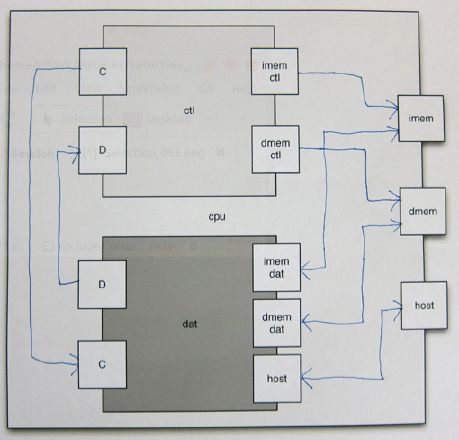
\includegraphics[width=0.8\linewidth]{figs/Bulk.png}

作为铺垫,比如现在已有如下Chisel代码:
\begin{scala}
	class RomIo extends Bundle {
		val isVal = Input(Bool())
		val raddr = Input(UInt(32.W))
		val rdata = Output(UInt(32.W))
	}
	class RamIo extends RomIo {
		val isWr = Input(Bool())
		val wdata = Input(UInt(32.W))
	}
	
	class CpathIo extends Bundle {
		val imem = RomIo().flip()
		val dmem = RamIo().flip()
		...
	}
	
	class Cpath extends Module {
		val io = IO(new CpathIo())
		...
		io.imem.isVal := ...
		io.dmem.isVal := ...
		io.dmem.isWr := ...
		...
	}
	class Dpath extends Module {
		val io = IO(new DpathIo())
		...
		io.imem.raddr := ...	
		io.dmem.raddr := ...
		io.dmem.wdata := ...
		...
	}
\end{scala}
这里用的也是面向对象的技巧来尽可能的复用代码。这样如果要编写一个将这些模块连接起来的顶层模块,Verilog肯定是一大堆的端口,然后是一大堆的信号,但是用Chisel语言,就可以简化为:
\begin{scala}
	class Cpu extends Module {
		val io = IO(new CpuIo())
		val c = Module(new CtlPath())
		val d = Module(new DatPath())
		c.io.ctl <> d.io.ctl
		c.io.dat <> d.io.dat
		c.io.imem <> io.imem
		d.io.imem <> io.imem
		c.io.dmem <> io.dmem
		d.io.dmem <> io.dmem
		d.io.host <> io.host
	}
\end{scala}
这种写法在Chisel的术语里叫做\textit{Bulk Connections}。		
	\end{multicols}

	那么上面两个例子所体现出的语言特性有没有实际工程上的作用,当然有。一个最为典型的例子就是AXI接口,首先AXI是有五个通道,而且非常的规整。所以抽取出五个通道的共通之处,写出一个基类。然后对五个通道如果有多余的端口可以扩展这个基类,只需要添加多余的端口就行了。更妙的是,不同组件通过AXI总线共连时,用bulk connection的写法,每连一对总线,只需要写一行代码。
	
	Chisel的威力还不止于此,再举一个例子,如果要实例化多个同样的module,Chisel可以用for loop,但是Verilog也可以做到,那就是generate的写法。但是如果仔细一看,Chisel的for loop翻译为
	Verilog可不是用generate的写法,而是有几个实例化几个。一开始觉得这个是笨方法,但是后来发现这是个很明智的选择。首先这些都是Chisel编译器干的事情,一点都没有增加人的工作负担,不用复制粘贴。其次这种写法的好处就是更加通用。这个更加通用体现在万一需求是要实例化多个略有差别的不同配置的module,比如前面的第一个例子要实例化100个不同功能的Filter,generate的写法显然不能胜任,但是Chisel编译的手法就能在for loop里面实现配置。然后编译好的Verilog文件真的就有100个不同配置的Filter。
	
	\subsubsection{Chisel test}
	Chisel沿袭了Verilog的传统,同一个语言可以用来设计电路也可以用来仿真电路,这样就不需要在两种语言之间做切换。而且由于Chisel承袭了Scala,而Scala承袭了Java,所以test设计的哲学思想也就自然顺承Java。从发展的角度来看,一开始的C\&C++没有严格的代码组织格式,test的设计也是如此,而且调试主要以真实的应用场景加上单步调试的GDB为主。到后来的Java对于代码的组织格式有了严格的要求,同时test的设计同样跟着代码的组织格式对每个模块进行了用例的assert测试。从而提出了一种比较系统的测试方法。引进的原因在于,用GDB跟着一个大系统单步调试往往效率是低下的,而把大系统拆分成一个个小的零件(其实也不用拆分,因为代码的组织格式就是按照一个个小的零件组织的),然后用一些包含edge case的用例来进行assert的测试就已经足够。这是一个非常好的想法,以至于后面的python更是凭借着解释语言的优势,可以以交互的方式对小零件单独测试,从而减少有这些小零件拼成的大系统的出bug数量和概率。所以Chisel自然有承袭了这一测试哲学。同时相比于Verilog中繁琐的测试代码编写,Chisel做了相应的简化与核心抽取。最大的一点改变就是不同于Verilog,在Chisel中不需要明确写出advance时钟一拍的逻辑,只需要简单写一句step(1)就能更新寄存器以及由寄存器驱动的组合逻辑。
 	\subsubsection{sbt 运行环境}
 	和Scala配套的build编译环境,和Java的maven类似,但其设计理念对于开发者更加友好。sbt负责管理编译的依赖关系,比如Chisel的库。
	\subsubsection{Firrtl}
	Firrtl是编译系统里面最重要的一层\chinesedash 中间表示层,代表了电路设计与翻译的标准~\cite{firrtl}。事实上,要理解Chisel的运行机制,确保生成的电路万无一失,如果直接看由Chisel生成的近似于Netlist的Verilog,是unreadable的。所以要了解Chisel的编译结果,就先要读Firrtl(Firrtl还有好几个层次,为的是一步一步将高级的构造语言简化)。另外一点是仿真的效率,因为最后生成的Verilog是slow to simulate,所以Chisel快速的仿真是基于Firrtl的。

\section{ISA}
设计一款具体的CPU,就要考虑到具体基于哪一个ISA。好在RISC-V和MIPS非常相似,所以实现了一个,另外一个很多功能部件都能够复用。如果一开始的设计就是尽可能的将微结构和ISA接耦合,那么只需要修改少量的逻辑即可。所以计划是先实现RISC-V,然后在移植到MIPS。架构是64位。
\subsection{MIPS}
一个最为熟悉但却依旧陌生的ISA。熟悉的部分是MIPS 32中的整数指令部分,以及CP0寄存器堆和特权模式处理机制。但是囿于最初并没有考虑到64位的需求和嵌入式系统压缩指令长度的需求,导致指令空间设计考虑不周,使得日后出现的microMIPS完完全全是不同的指令集和MIPS32/64不兼容。MIPS的64位部分、压缩长度指令部分以及浮点部分对我来说是陌生的。
\subsection{RISC-V}
RISC-V作为一个2010年以后才出现的ISA,完全有着历史经验的优势,可以充分的借鉴前人设计的优缺点。所以32位,64位,压缩变长指令集都是统一的一个指令集下的不同形式。ISA的演进已经有40多年的历史,就目前而言逐渐趋向于收敛,而且RISC-V设计时也考虑到要有极强的可拓展性以便日后之需。同时RISC-V的设计模式也和之前所以增量式指令集不同:

不同于几乎所有的先前的ISAs,RISC-V是模块化的。核心是基础的ISA\chinesedash RV32I,足以运行整个软件栈。RV32I是被冻结的并且永远不会改变,是稳定的。然后其他的扩展功能的指令以可选的方式可添加。~\cite{reader}

那么相比于MIPS,RISC-V有什么特点呢?
\begin{enumerate}
	\item 首先用户态的对比。
	
	MIPS有延迟槽这么一条设计。这个被后来证明不是一个好主意,因为其设计的哲学就有问题,延迟槽实际上代表着ISA和设计实现的不独立,这是非常糟糕的。比如单发射五级流水有延迟槽就非常nice,不用停流水或者做转移猜测。但是对于多发射的实现呢?一条延迟槽不够了。这就是ISA和设计实现不独立的后果。在其他细节上,RISC-V取缔了HILO,但是32位的乘法和除法结果都是64位的,怎么解决。RISC-V选择软件来解决\chinesedash 代码上写两条指令,一条得到低(商)32位,一条得到高(余数)32位,存在两个不同的寄存器里。那么这个设计有没有设计与ISA不独立之嫌呢?我觉得没有,首先在32位的架构下,寄存器都是32位的,如果要用到乘除法的结果,也是要通过mfhi,mflo指令来操作的。既然如此ISA就规定要算出乘除法的完整结果,就是需要两条指令,至于微结构实现要怎么做,那就看微结构的设计者,可以老老实实算两次,也可以一旦发现有连续的两条算高低位的指令,就做一次运算。如果恰好碰到中断之类的,就只好自认倒霉,再算一次了。同时算术指令中也取缔了overflow例外,将其移到了软件实现:~\cite{user}
	\begin{scala}
		add t0, t1, t2
		slti t3, t2, 0
		slt t4, t0, t1
		bne t3, t4, overflow
	\end{scala}
	
	在RISC-V中较于MIPS还有两大亮点:
	\begin{itemize}
		\item 不像MIPS用LWL,LWR来支持地址的非对齐访问。由于RISC-V指令可以是变长的,所以非对齐的访问是自然支持的。
		\item RISC-V支持pc相关地址访问。在RISC-V中有这样一条指令 AUIPC(add upper immediate to pc),该指令从指令中的20位立即数的基础上第12位填充上0构成32位偏移量与当前的PC相加结果哦存到rd寄存器中。
	这样做的好处在于代码数据整体拷贝时,不用改动任何东西就能够运行原来的这段程序,因为相对位置没有改变。
	\end{itemize}
	如下是用到AUIPC的场合:~\cite{user}
		
	\begin{tabular}{l l l}% centered columns (4 columns)
		\hline                        %inserts double horizontal lines
		Meaning & Base Instruction(s) & Pseudoinstruction %inserts table 
		%heading 
		\\ [0.5ex] \hline Load address & \begin{tabular}{@{}l@{}} \tt auipc rd, symbol[31:12] \\ \tt addi rd, rd, symbol[11:0] \end{tabular} & \tt la rd, symbol
		\\ \hline Load global & \begin{tabular}{@{}l@{}} \tt auipc rd, symbol[31:12] \\ \tt l\{b|h|w|d\} rd, symbol[11:0](rd) \end{tabular} & \tt l\{b|h|w|d\} rd, symbol
		\\ \hline Store global & \begin{tabular}{@{}l@{}} \tt auipc rd, symbol[31:12] \\ \tt s\{b|h|w|d\} rd, symbol[11:0](rd) \end{tabular} & \tt s\{b|h|w|d\} rd, symbol
		\\ \hline Floating-point load global & \begin{tabular}{@{}l@{}} \tt auipc rd, symbol[31:12] \\ \tt fl\{w|d\} rd, symbol[11:0](rd) \end{tabular} & \tt fl\{w|d\} rd, symbol
		\\ \hline Floating-point store global & \begin{tabular}{@{}l@{}} \tt auipc rd, symbol[31:12] \\ \tt fs\{w|d\} rd, symbol[11:0](rd) \end{tabular} & \tt fs\{w|d\} rd symbol
		\\ \hline Call far-away subroutine & \begin{tabular}{@{}l@{}}
			\tt auipc x6, offset[31:12] \\
			\tt jalr x1, x6, offset[11:0]
		\end{tabular} & \tt call offset
		\\ \hline Tail call far-away subroutine & \begin{tabular}{@{}l@{}}
			\tt auipc x6, offset[31:12] \\
			\tt jalr x0, x6, offset[11:0]
		\end{tabular} & \tt tail offset
		\\[1ex] \hline %inserts single line
	\end{tabular}
	\item 其次是特权态的对比
	
	MIPS的特权态的管理用到的是Coprocessor 0,负责对虚实地址和例外处理进行管理。记录特权状态的寄存器的地址空间仅有区区5位32个。但是RISC-V却有12位的地址空间,最多4096个寄存器可用。下图就是Control and Status Registers(CSR) 的地址空间的分配:~\cite{privileged}
	\begin{figure}[H]
		\centering
		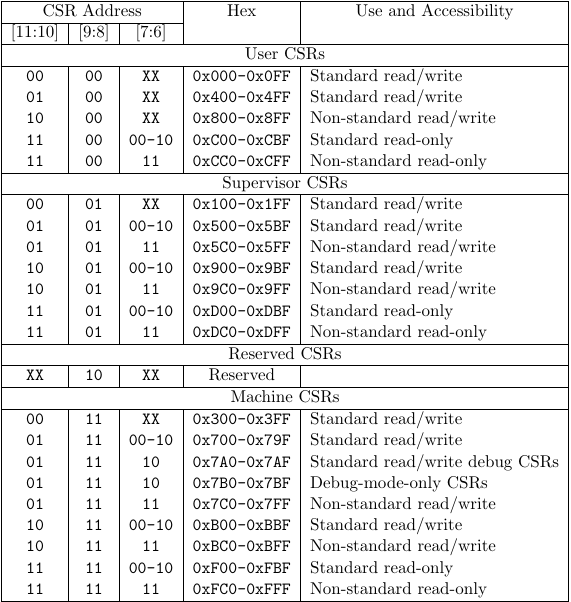
\includegraphics[width=0.4\linewidth,height=0.26\textheight]{figs/CSR.png}
	\end{figure}
	
	虽然RISC-V在操作系统等大型软件上的经验还不如MIPS雄厚,而且在手册上也明确说是\textit{draft},但是其特权态的规范在这几年快速地发展,运行像Linux这样的操作系统已经是绰绰有余了。
	
	用模型的角度来分析,特权态也不过是在用户态模型之上更高等级的状态(state)。而这个状态是由寄存器(Control and Status Registers)来维护的。同时整个模型通过输入特权态指令来改变以及管理这些状态。那么怎么衡量一个ISA对于不同等级模式的刻画干不干净,就要看这个state以及state的变化规不规整。从这个角度而言,RISC-V作为一个参考了当今软件的运行模式的ISA,是比MIPS更干净的。首先RISC-V将处理器的状态分为了3个等级(Mode):~\cite{privileged}
	\begin{figure}[h]
		\centering
		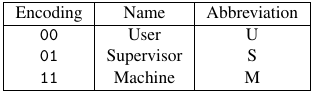
\includegraphics[width=0.3\linewidth]{figs/mode.png}
	\end{figure}

	而这3个等级的2 bits编码均体现在Privileged Instructions的编码(用户态的指令不用这么编码是因为无论哪个等级都可以执行这些指令,而且省去这两位能够增加3倍的指令编码空间)和寄存器空间的编码。这样什么等级的指令执行在什么等级状态下CPU上,要修改什么等级的寄存器,都有非常干净的规定。
	
	在三个等级中最为基础的就是Machine Mode。而M等级中基础的控制寄存器其实基本上和MIPS CP0中的寄存器是一一对应的。如下列举几个:~\cite{privileged}
	\begin{itemize}
		\item {\tt mtvec}, \textit{Machine Trap Vector} 存储例外的跳转地址。
		\item {\tt mepc}, \textit{Machine Exception PC} 存储例外发生的指令PC
		\item {\tt mcause}, \textit{Machine Exception Cause} 指示例外发生的原因与类型
		\item {\tt mie}, \textit{Machine Interrupt Enable} 列举了哪些例外处理器会相应,哪些会忽略
		\item {\tt mip}, \textit{Machine Interrupt Pending} 列举当前pending住的中断
		\item {\tt mtval}, \textit{Machine Trap Value} 与MIPS中的BADADDR功能一致
		\item {\tt mscratch}, \textit{Machine Scratch} 一个指令长度的数据临时存储
		\item {\tt mstatus}, \textit{Machine Status}
		与MIPS中的STATUS功能类似
	\end{itemize}
	这里比较有特色的寄存器是mscratch。如果编过MIPS的Linux内核,就会知道比如context switch和TLB的例外处理都需要用到K0和K1寄存器,这两个寄存器就是专门留给操作系统用于临时存储数据用的。虽然这样很高效,但是白白浪费了两个通用寄存器。另外一方面像context switch和TLB的例外处理是与M等级有关的,所以从设计的哲学上来讲也应该归特权级别的寄存器管理而不是通用寄存器。这也是RISC-V更为干净的一种体现。
	
	在特权态中最为重要的内存管理,而一个最基本的考虑就是用户态不可信赖的程序要严格限制其只能访问到自己内存范围的内容。所以RISC-V要想做好,也必须在这方面下功夫。首先RISC-V在M等级和U(User)等级之间设计了一种内存保护机制:Physical Memory Protection (PMP)。这样M等级就可以配置U等级程序能够访问的内存区域以及访问的权限。
	\begin{figure}[H]
		\centering
		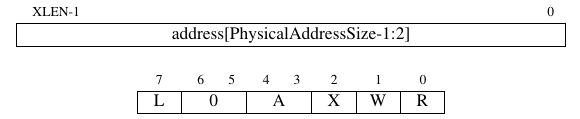
\includegraphics[width=0.7\linewidth]{figs/PMP1.png}
		\end{figure}
	上图~\cite{privileged}的上半部分是PMP寄存器, 一般处理器会实现8-16个这样的寄存器。
	而这个configuration(上图的下半部分)也是存储在寄存器里的(R代表读,W代表写,X代表执行,A代表PMP使能,L代表locked),见下图:~\cite{privileged}
	\begin{figure}[H]
		\centering
		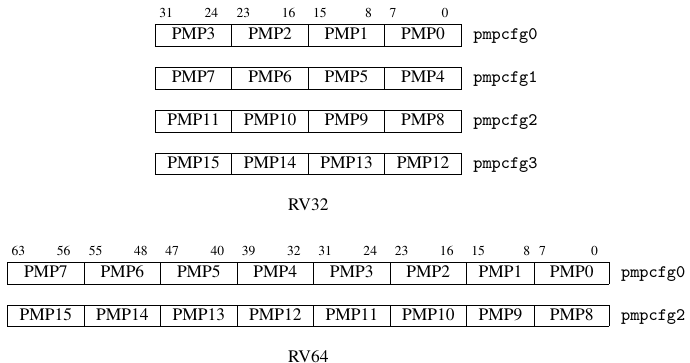
\includegraphics[width=0.7\linewidth]{figs/config.png}
	\end{figure}
	这个configuration寄存器授权或者禁止读写执行。当处理器在U-mode试图想要取指或者执行load和store请求时,其地址将会被和PMP中的地址进行比较,如果地址大于等于i号PMP而小于i+1号PMP。那么i+1号的PMP对应的configuration寄存器将会规定访问内存的模式,如果实际的访问方式逾越了configuration里的规定,就会引发例外。~\cite{privileged}
	
	对于嵌入式系统,PMP机制能够非常有效的对内存实行保护。但是其有两个缺点使之不适合更为复杂的系统和通用计算,分别是:
	\begin{itemize}
		\item 只支持最多16个内存区域,不能扩展性
		\item 这些区域都是连续的,有点像操作系统早期的\textbf{段}的概念。所以对内存的片段化支持不好。这也正是段的缺点
	\end{itemize}
	所以RISC-V的ISA必须支持基于页的虚拟内存机制。而这个特征直接主导了介于M等级和U等级中间的等级\chinesedash supervisor mode(S等级)。
	
	理论上来讲,RISC-V中所有的例外都是要将处理器的控制权转移到M等级的例外handler。但是大多数的Unix系统的例外需要invoke系统内核,而系统内核又是运行在S等级的。如果先由系统将用户进程切换到内核,然后再由CPU将内核切换到M等级处理 (或者说M等级要重新路由到S等级),~\cite{reader}
	这样效率就会大大降低。所以RISC-V提供了例外授权机制(exception delegation mechanism),这样中断和同步例外就能bypass M等级,选择性的授权给S等级。而CSR寄存器 {\tt mideleg }(Machine Interrupt Delegation)和{\tt medeleg }(Machine Exception  Delegation) 正是这个机制的载体。对应于{\tt mip }和 {\tt mie }寄存器的exception code,举例来说,{\tt mideleg[5]} 对应于S等级的时钟中断,如果被置上,S等级的时钟中断将会把控制权转移到S等级的exception handler上而不是M等级的exception handler;同样,如果{\tt mideleg[15]}被置上,则会将store page faults授权给S等级来处理。不过需要注意的是,在某等级发生的例外永远不会转移控制权给更低的等级,具体来说就是在M等级发生的例外就只能M等级来处理;S等级发生的例外可能由M等级或者S等级来处理,取决于delegation configuration,但永远不会是U等级。
	RISC-V的分页方案命名方式为\textbf{SvX},比如32位的虚拟地址就是Sv32, 其支持4GiB的虚拟地址,有两级页表,分别是是$ 2^{10} $个 4MiB的页表,然后每个页表又有$ 2^{10} $个4KiB的基页。下图是Sv32和Sv39的page-table entry(PTE)~\cite{reader}
	\begin{figure}[H]
		\centering
		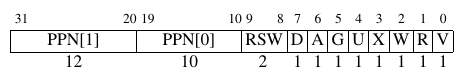
\includegraphics[width=0.5\linewidth]{figs/Sv32.png}
		\captionsetup{labelformat=empty}
		\caption{An RV32 Sv32 page-table entry (PTE)}
		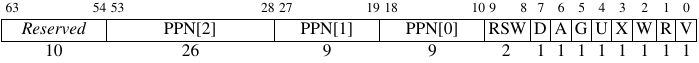
\includegraphics[width=\linewidth]{figs/Sv39.png}
		\captionsetup{labelformat=empty}
		\caption{An RV64 Sv39 page-table entry (PTE). }
	\end{figure}
	Sv39是$ 2^9\times 2^9\times 2^9 \times 2^{12} $的模式,所以是3级页表。
	% \begin{commentary}
	% 	The other RV64 paging schemes simply add more levels to the page table. Sv48 is nearly identical to Sv39, but its virtual-address space is 29 times bigger and its page table is one level deeper.
	% \end{commentary}
	S等级用satp(Supervisor Address Translation and Protection) S-mode的CSR来管理分页系统。
	\begin{figure}[H]
		\centering
		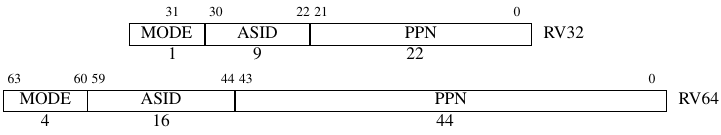
\includegraphics[width=0.7\linewidth]{figs/satp.png}
	\end{figure}
	\begin{figure}[H]
		\centering
		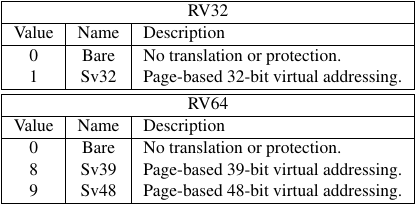
\includegraphics[width=0.4\linewidth]{figs/MODE.png}
		\captionsetup{labelformat=empty}
		\caption{The encoding of the MODE field in the satp CSR.~\cite{privileged}}
	\end{figure}
	在处理器进入S等级之前,M等级首先会写0到satp寄存器,禁止分页;然后等到进入S等级在设置了页表之后,S级的软件优惠重新写satp寄存器
	最后是虚拟地址转实际地址的过程,注意到如果操作系统修改了page table,那么就要用sfence.vma指令来flush相应的TLB entry。
\end{enumerate}

\section{RTL模型与逻辑}
RISC架构的CPU,可以看做一个以指令和load作为输入,修改内部状态,并通过store对外界反馈的器件,这里的内部状态state是由程序计数器PC,通用寄存器,特权态所需的Control and Status Registers所构成的。同时所做的运算基本上是二规约的,也即两个操作数变换得到一个结果。在冯诺依曼体系结构下,大致的流程是CPU通过取指器件取回来指令并修改下一拍的PC;同时将取回来的指令进行译码,转化为内部编码。如果是算数指令,等待操作数的准备就绪然后一起发送到运算部件,最后将结果存储入寄存器中,如果是特权指令,修改或者读取相应的Control and Status Register。下面首先对一些经典的微处理器设计进行分析,然后对关键的组件进行初步的设计考虑。

\subsection{可供参考的实例}
	\subsubsection{Alpha 21264}
		Alpha 21264是处理器历史上的经典之作。下面就从\textit{THE ALPHA 21264 MICROPROCESSOR}~\cite{alpha}这篇技术报告里摘要出来其微结构的设计的highlight。
		
		下图是Alpha 21264的逻辑框图:~\cite{alpha}
		\begin{figure}[H]
			\centering
			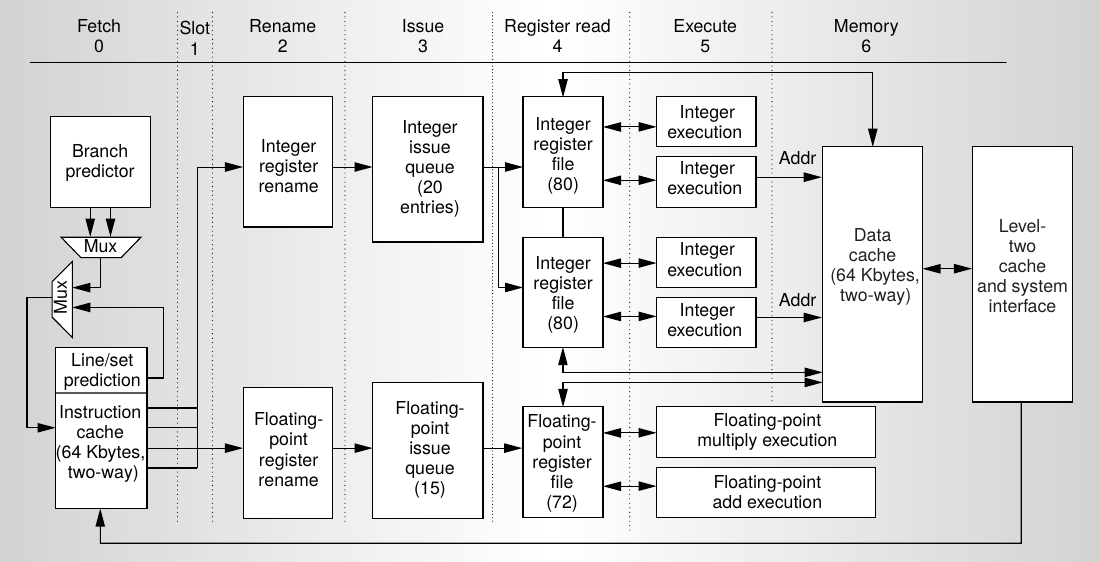
\includegraphics[width=0.8\linewidth]{figs/21264.png}
		\end{figure}
	\begin{multicols}{2}
	\begin{enumerate}
		\item \textbf{取指}。21264为了提高取指的效率,采用了两种方法,一种是line and way prediction,另一种是branch prediction。由于21264的icache采用的是两路组相连,一种方案是把line对应的两个way都读出来,然后在mux一下,不过这样可能最长路径就会卡在取回指到译码上,而且可拓展性也不好,如果要实现一个一次取四条指令的CPU,四选一就会更加影响时序。采用预测技术由于猜得准,猜错代价小,所以提高了取指模块的性能。
		
		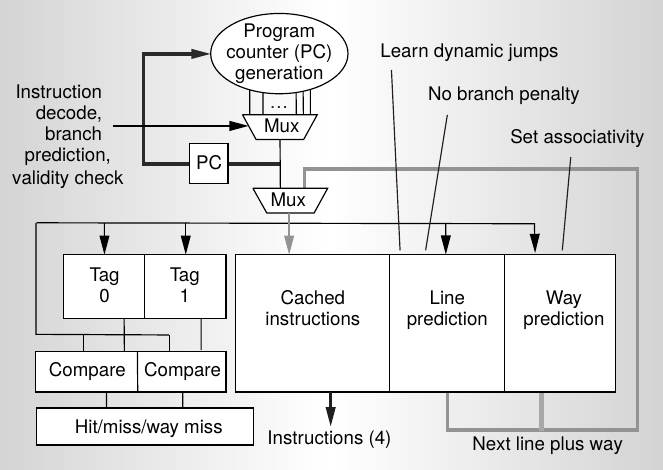
\includegraphics[width=\linewidth]{figs/prediction.png}
		
		这幅图~\cite{alpha}的大致解读是处理器基于PC加上各种预测手段取出下一组指令,与此同时完成上一组取回来指令的有效性检查。训练的line predictor对于使用动态链接库的代码有好处。这是因为对于非直接(subroutine) jump, 这个jump一定会跳,所以没有Branch predictor什么关系,但是在复杂的乱序pipeline中要计算出jump的地址至少就需要8拍,所以cache行的预测是非常有必要的,以提供连续的指令流。
		
		而分支猜测同样非常重要,猜错与不猜都是7拍的损失。
		21264实现了复杂的转移猜测机制,这个机制会动态的选择局部历史和全局历史的结果来预测跳转的方向。~\cite{alpha}
		两种方法的结合比任何一种用更大的表的单一方法的准确率都要高。
		
		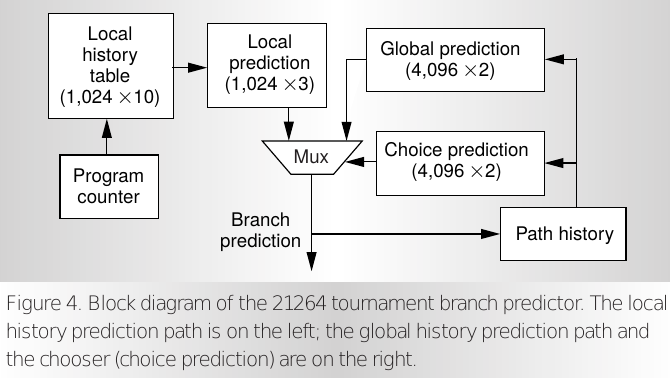
\includegraphics[width=\linewidth]{figs/branch.png}
		
		\item \textbf{乱序执行}。虽然取回来是4条指令,但是在保留站内却是6条指令发射,四条整数指令,两条浮点指令。由于中间寄存器(internal register)需要指示用户可见的寄存器的对应关系,所以寄存器重命名是一个content-addressable memory(CAM)操作。除了各31个可见的用户可见的integer和float-point寄存器,还有额外的41个浮点寄存器和41个整数寄存器可以用来存放乱序得到的指令的结果。
		
		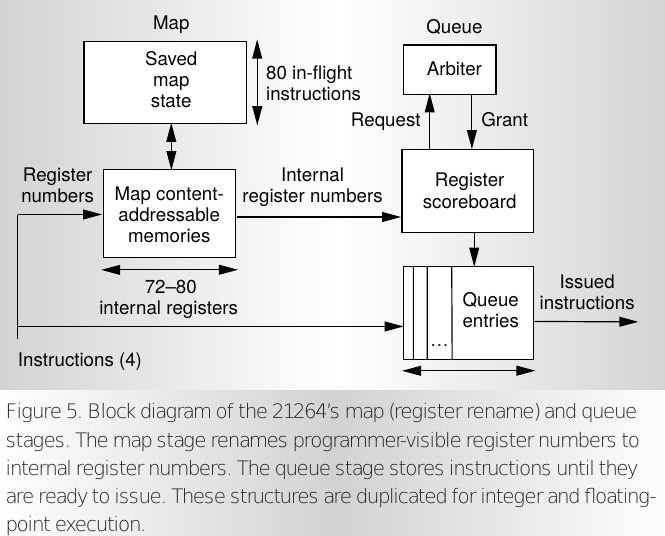
\includegraphics[width=\linewidth]{figs/rename.png}
		
		发射的细节上,微结构上有一个20-entry的integer queue和一个15-entry的float-point queue。发射的是那些操作数都已经准备好的指令。如何知道操作数已经准备好了?21264根据每种指令采用了计分板。
		% \begin{quote}
		% 	Using register scoreboards based on the internal register numbers. These scoreboards maintain the status of the internal registers by tracking the progress of single-cycle, multiple-cycle, and variable-cycle memory load) instructions. When functional-unit or load-data results become available, the scoreboard unit notifies all instructions in the queue that require the register value. These dependent instructions can issue as soon as the
		% 	bypassed result becomes available from the functional unit or load. 
		% \end{quote}
		同时队列由两个arbiter来决定填入新的指令。
		
		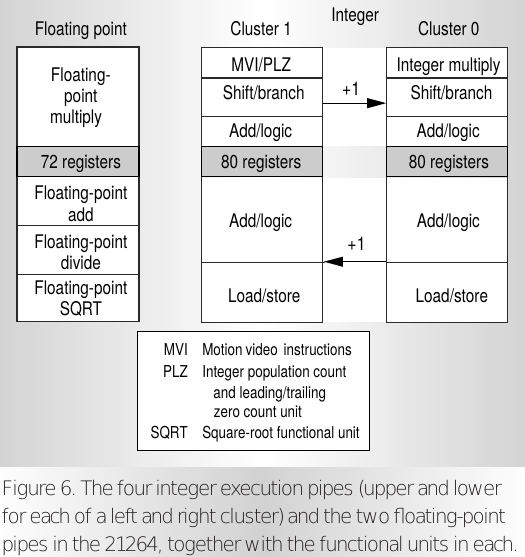
\includegraphics[width=\linewidth]{figs/pipeline.png}
		
		如上图~\cite{alpha},alpha21264的流水线设计使用了6条execution piplines,特别是整数的流水线设计了两个cluster。设计的基本考虑是要和前面所提到的issue queue配套。cluster使得设计更加简单和快速,即使它会有额外的时钟开销去在各个cluster中广播结果。采用动态仲裁哪个cluster执行指令。
		
		% \begin{commentary}
		% 	This clustering makes the design simpler and faster, although it costs an extra cycle of latency to broadcast results from an integer cluster to the other cluster. The upper pipelines from the two integer clusters in the above figure are managed by the same issue queue arbiter, as are the two lower pipelines. The integer queue statically slots instructions to
		% 	either the upper or lower pipeline arbiters. It then dynamically selects which cluster to execute an instruction on, left or right.
		% \end{commentary}
		\item \textbf{retire \& commit}. 指令结果的commit是顺序的,这也意味着两点:
		\begin{itemize}
			\item 在指令开始执行之后,要等到之前的指令都retire完了并且保证自身没有例外发生才可以retire。
			%After an instruction starts executing, it can retire whenever all previous instructions have retired and it is guaranteed to generate no exceptions. 
			\item 物理寄存器要等到对应的指令提交retire,才能成为用户可见的。
			%The register only becomes part of the user-visible (architectural) register state when the instruction retires/commits.
		\end{itemize}
		\item \textbf{exception handling}. 21264实现的是精确例外,也就是说如果老的指令发生了例外,年轻的指令不会改变处理器的state。但是由于处理器是乱序执行的,所以完全有可能出现年轻的处理器先改变了internal register的state。所以必须有回滚机制,也就是在指令未retire之前,要记住原来存储的值。retire机制维护一个80条指令的inflight window并且可以一拍内retire最多11条指令并可以维持每拍8条指令的retire速率。
		\item \textbf{memory system \& bus interface}.
		每拍支持两条从整数流水线出来的内存访问。同时可跟踪32条in-flight loads(32-entry load queue),32条in-flight stores(32-entry store queue)和8条in-flight(instruction或者data) cache miss请求。dcache是64KB两路组相连的配置。因为每一拍可以支持两次内存访问,所以dcache的主频是CPU主频的2倍。~\cite{alpha}
		
		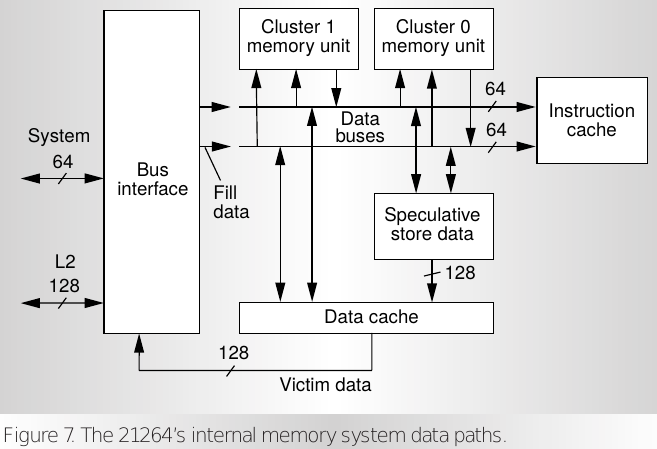
\includegraphics[width=\linewidth]{figs/memory.png}
		图中两条64-bit data buses是internal memory system的核心。store首先会通过数据bus将其数据先转移至store buffer中。并且store可以forward数据到后续的load操作当store的数据依然在数据buffer中。实际上这个store data buffer起着内存的重命名功能。
		% \begin{commentary}
		% 	The LDQ (STQ) positions loads (stores) in the queue in fetch order, although they enter the queue when they issue, out of order. Loads exit the LDQ in fetch order after the loads retire and the load data has been returned. Stores exit the STQ in fetch order after they retire and dump into the data cache.
		% \end{commentary}
		为了解决read-after-read, read-after-write, write-after-read和write-after-write的hazards,21264使用了双端口的地址CAMs。~\cite{alpha}
		
		同时,memory system中还包含了MAF,简言之就是能够自动合并不同读写相同block的请求。
		
		internal memory system将MAF传给bus interface unit(BIU),然后由BIU来沟通off-chip的L2 cache以及其系统的其他部分,值得注意的是BIU管理者dcache的内容。所以最后它会收到来自系统的cache probes,然后进行必要的cache一致性的操作,最后相应系统。
		% \begin{commentary}
		% 	The 21264 implements a write-invalidate cache coherence protocol to support shared-memory multiprocessing.
			
		% 	The total of eight in-flight MAFs and eight in-flight victims provide many parallel memory operations to schedule for high SRAM and DRAM efficiency. This translates into high memory system performance, even with cache misses.
		% \end{commentary}
	\end{enumerate}
	\end{multicols}	
	\subsubsection{MIPS r10000}
	MIPS r10000也是微处理器设计中广为人知的经典之作。如下是其微结构的逻辑框图:~\cite{mips}
	\begin{figure}[H]
		\centering
		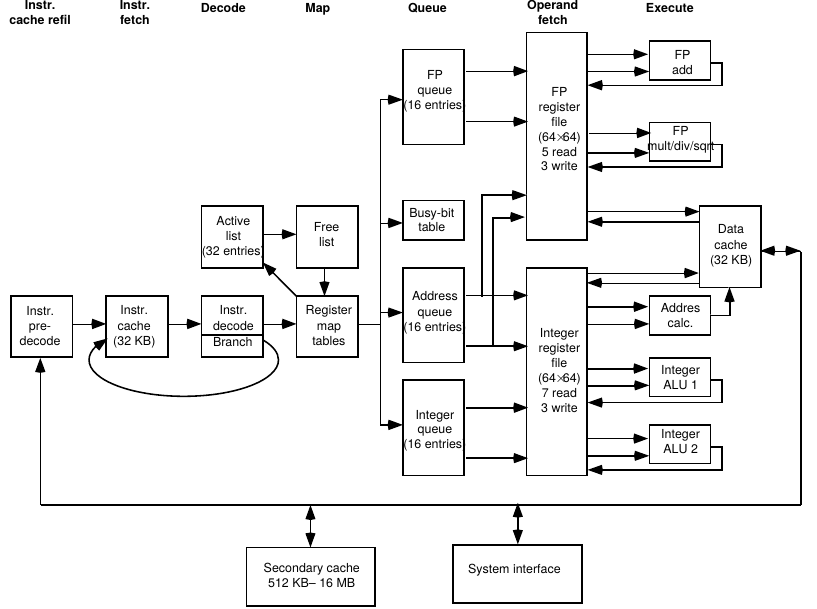
\includegraphics[width=0.6\linewidth]{figs/MIPSr10000.png}
	\end{figure}
	\begin{multicols}{2}
		\begin{enumerate}
			\item \textbf{取指}。r10K一拍内能取4条指令。如果指令因为是structural hazards 或者指令本身是special instructions,那么将会被搁置在8-word的instruction buffer里而先不会被译码。
			\item \textbf{转移猜测}。用2-bit 512 entry BHT,有4个entry branch stack存储着alternate branch address和integer and FP register map tables的副本。意思应该是支持4次转移猜测而不阻指令流。如果预测错了,进行Mispredicted branches的处理,首先立刻恢复state,并且依据alternate branch address来取指。为了取消掉取错的指令,r10K每条指令都标记着4 bit branch mask,对应的是哪一次分支预测后所取的指令。~\cite{mips}
			
			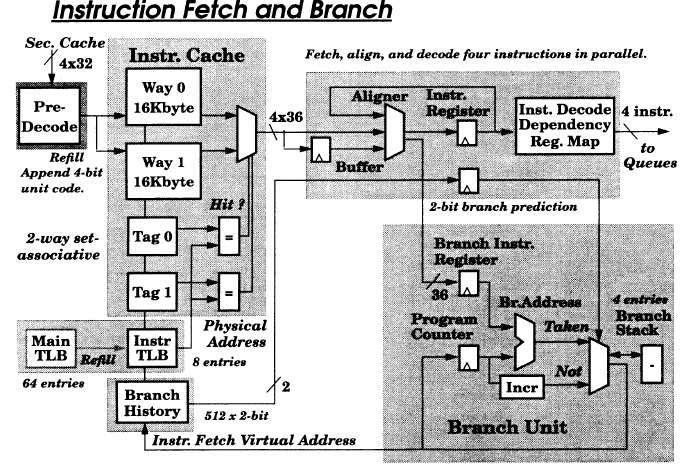
\includegraphics[width=\linewidth]{figs/10Kbranch.png}
			
			\item  \textbf{寄存器重命名}。MIPS逻辑的通用寄存器空间有5位,r10K物理寄存器空间有6位,也就是最多64个。能够消除WAR and WAW hazards。同时维护着$ 33\times 6 $ bit RAM的整数寄存器map表和$ 32\times 6$bit RAM的浮点寄存器map表。r10K还有32 entry FIFOs (four parallel, eight-deep)~\cite{mips}
			的Free List,里面维护的信息是当前未分配的物理寄存器号。与此对应的是Active list。所有in-flight的指令都被记录在32-entry的FIFO (four parallel, eight-deep) 中,所以为每一条指令提供了了5-bit的ID。操作起来像reorder buffer,如果运算单元完成了指令的运算,将会发送tag到Active list,然后将对应entry的done bit置上。每个entry中还存储了逻辑的目的寄存器号和旧的物理寄存器号。同时r10K支持精确例外,当例外发生,例外指令的后续指令不会被graduate,处理器也会从the active list中恢复旧的映射关系。
			
			这里是性能的直接体现,前文中的Alpha 21264最多支持80条指令乱序执行,而MIPS r10K是32条,差距还是比较明显的。
			
			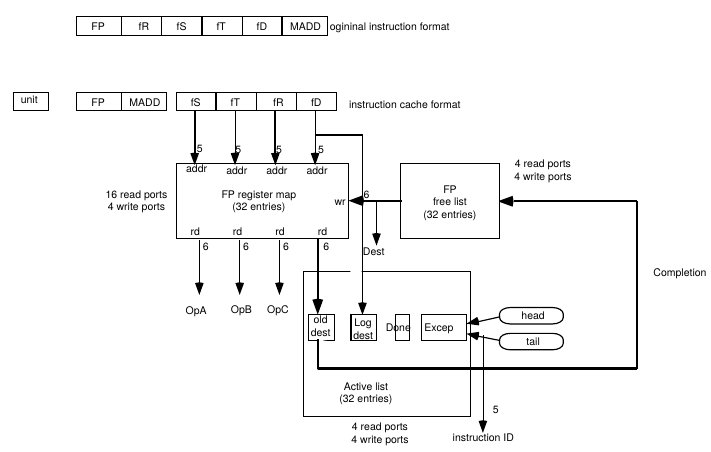
\includegraphics[width=\linewidth]{figs/10Krename.png}
			\item \textbf{发射队列}。有三个队列,分别是Integer,Address和Float-point. 队列在整个CPU的关键路径上,在译码的时候分配entries。三个队列的配置相似,都是16-entries,每个entry有10个16 bit comparators来处理 RAW hazards。~\cite{mips} 不同之处在于Interger和FP no order的,言下之意是如队列是从尾进,出队列issue则是没有绝对次序的,只有在大于运算流水能够允许的最大发射数量的时候才会看次序。但是访存的队列就是有order的。严格按照次序发射进行地址运算然后访问内存。以Integer Queue为例,有下图:~\cite{mips}
				
			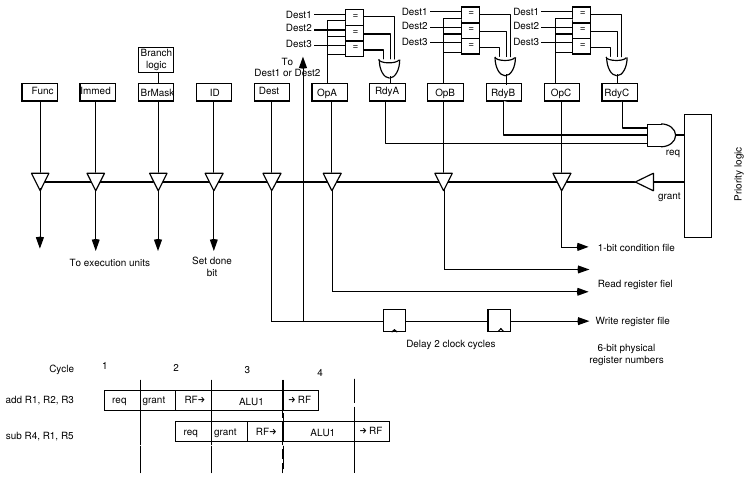
\includegraphics[width=\linewidth]{figs/r10Kqueue.png}
			
			\item \textbf{指令执行和流水}。可以用如下框图和时序图来概况r10K的行为:~\cite{mips}
			
			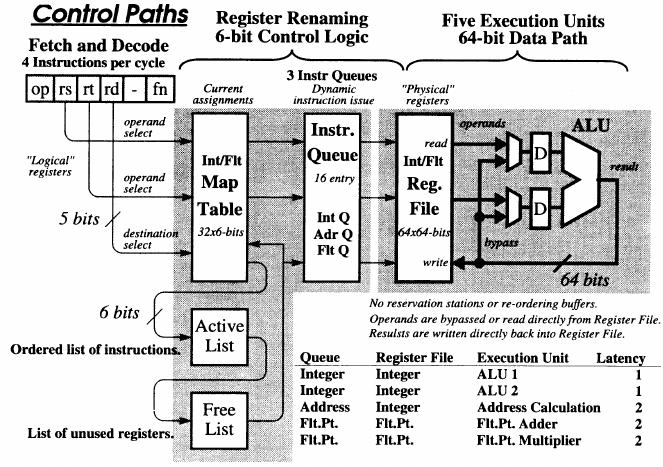
\includegraphics[width=\linewidth]{figs/execute.png}
			
			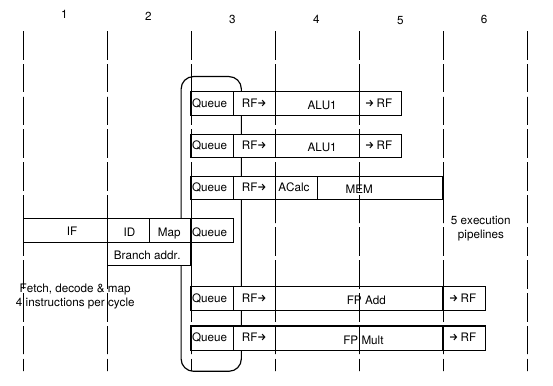
\includegraphics[width=\linewidth]{figs/r10Kpipeline.png}
			
			\item \textbf{Memory Hierarchy}.
			32KB, 2路,128B line size(16条64位的指令)的icache;
			
			TLB的结构是有64个entries,每个entries 2pages,如果每个page有4KB,那么能够快速转化的虚拟地址是1MB;
			
			dcache是32KB,2-way,64B line size, writeback。还有支持如下特性:~\cite{mips}
			\begin{itemize}
				\item 2路 interleaved 取数存数以及cache充填来提高带宽。
				\item 非阻塞outstanding支持4条访存请求。
			\end{itemize}
		
			L2 cache是128b的interface,可配置容量512KB-16MB,采用pseudo 2-way SA using 8 Kb MRU table.~\cite{mips}
			
			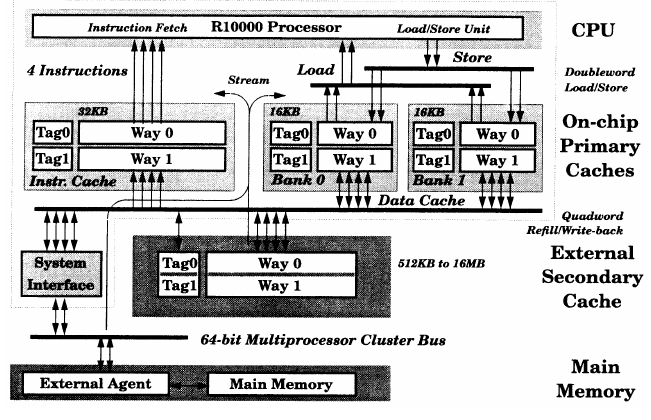
\includegraphics[width=\linewidth]{figs/r10Kmemory.png}
		\end{enumerate}
	\end{multicols}
    \subsubsection{BOOM}
    % \begin{commentary}
    % 	BOOM is heavily inspired by the MIPS R10k and the Alpha 21264 out–of–order processors. Like the R10k and the
    % 	21264, BOOM is a unified physical register file design (also known as “explicit register renaming”).
    % \end{commentary}
	BOOM是和RISC-V一起开源的一款superscalar和out-of-order处理器核。
	
	BOOM的设计者是和我一样的学生,所以同样参考的是最为经典MIPS R10k和Alpha 21264。~\cite{Celio:EECS-2017-157}
	BOOM的版本经历了两代,下图是两代的对照:
	\begin{figure}[H]
		\centering
		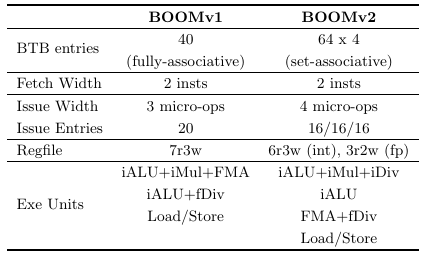
\includegraphics[width=0.4\linewidth]{figs/BOOMv1v2.png}	
		\captionsetup{labelformat=empty}
		\caption{BOOMv1,v2配置对照表~\cite{Celio:EECS-2017-157}}
	\end{figure}		
	但是注意到BOOM其实是高度可配置的generator,换言之前面几个参数都是可以配置的。
	\begin{figure}[H]
		\centering
		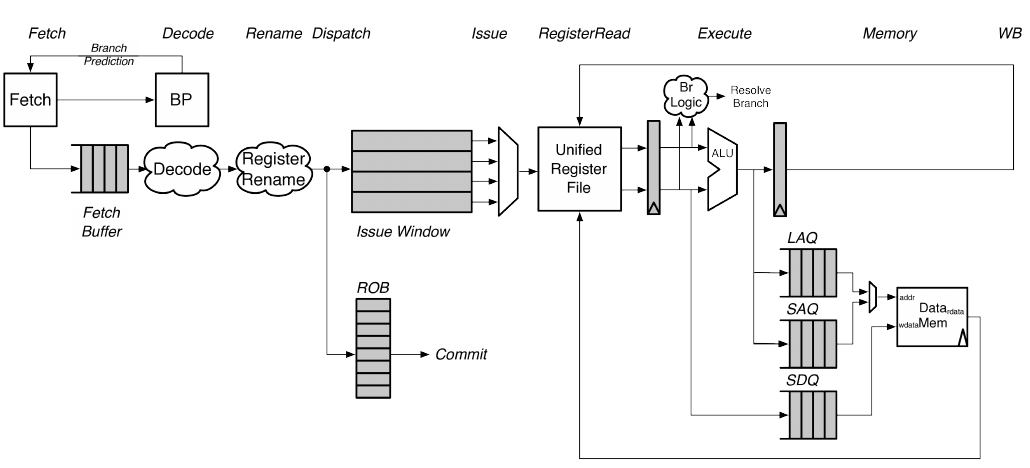
\includegraphics[width=0.73\linewidth]{figs/BOOM.png}
		\captionsetup{labelformat=empty}
		\caption{BOOMv1的逻辑框图~\cite{Celio:EECS-2017-157}}	
	\end{figure}
	如下是BOOMv2和v1的结构对照图:
	\begin{figure}[H]
		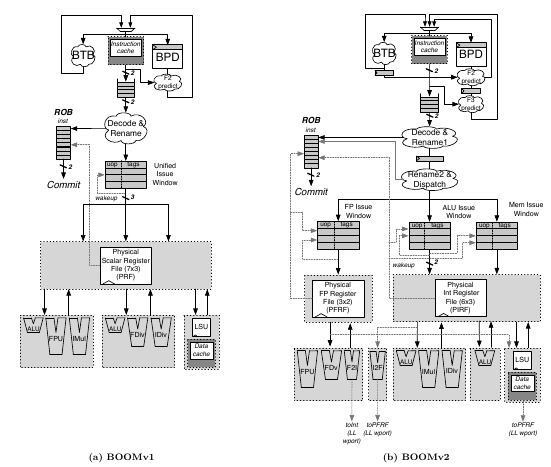
\includegraphics[width=0.9\linewidth]{figs/Boomv1v2.png}
		\captionsetup{labelformat=empty}
		\caption{BOOMv1 and BOOMv2的datapath对比。v2的发射窗口和物理寄存器都是分布式的并且在取指和寄存器重命名阶段多加了一拍。~\cite{Celio:EECS-2017-157}}	
	\end{figure}
	\begin{multicols}{2}
		\begin{itemize}
			\item \textbf{BOOMv1}(下面简称v1)
						
			v1的IPC达到 3.91 CoreMarks/MHz (和A9相似配置)和ARM Cortex-A9的IPC相当,按我的以前的经验,单发射五级静态流水最多可以做到3出头点的分数(也就是IPC接近于1)。所以第一代IPC不错,快了差不多33\%。主频方面,用IBM 45 nm SOI的工艺可以达到1.5GHz, the SRAM access 将会成为 the critical path~\cite{Celio:EECS-2017-157}。感觉言下之意就是不是他设计不行,奈何工艺不好。如下是BOOMv1
			文档中的各款处理器的性能对比图~\cite{Celio:EECS-2017-157}:
			
			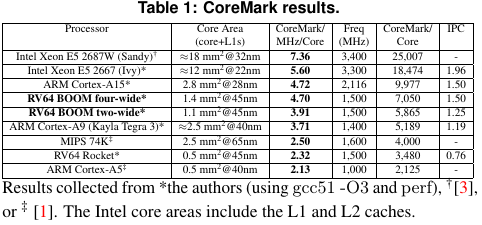
\includegraphics[width=\linewidth]{figs/result.png}
			
			这里有一个我没有搞清楚的地方是two-wide和four-wide,文档里没有交代,我估计是发射的宽度,也即从保留站里每拍至多发射多少条指令去执行流水线上执行。
			
			v1效仿MIPS R10K的设计,采用了6级流水 -- fetch, decode/rename, issue/register-read, execute, memory, and writeback。对应分支跳转的预测在分支指令被译码的后一拍执行。同时物理寄存器是unified的,integer和float-point寄存器统一在一起,包括运算单元也是整数部件和浮点部件混合在一起.~\cite{Celio:EECS-2017-157}
			\item \textbf{BOOMv2}(下面简称v2)
			现有的文档更多的是介绍第二代版本。所以v1和v2的比较以及整个BOOM的微结构设计都放在这里说明。首先需要交代的一点就是相比于v1, v2缩短了关键路劲的延迟,但是IPC却比v1降低了20\%.~\cite{Celio:EECS-2017-157}
			\begin{enumerate}
				\item \textbf{取指}。包括转移猜测在内,整个提供指令流的部分被成为frontend. BOOM采用了3中手段来提高转移猜测的准确率。
				\begin{enumerate}
					\item Branch Target Buffer (BTB) 维护的是一个PCs到branch target的映射表,用PC地址索引查表然后对比tag,命中则做出预测。同时有一些hysteresis bits来帮助做出taken/not-taken的决定。BTB是非常耗费资源的结构,大概要20 bits的tag和整个64 bits的target(整个架构是64位)
					\item Return Address Stack (RAS) 预测函数的返回地址。函数的调用和返回可以用栈的结构来刻画。
					\item Conditional Branch Predictor (BPD) 针对分支决定跳与不跳的预测,不会存储耗费资源的branch targets,而是通过取回来的分支指令计算得到跳转的地址。一种常见的BPD是global history predictor。通过跟踪钱N次跳转的历史,并将这个历史hash到预测表中。
				\end{enumerate}
			\begin{figure}[H]
			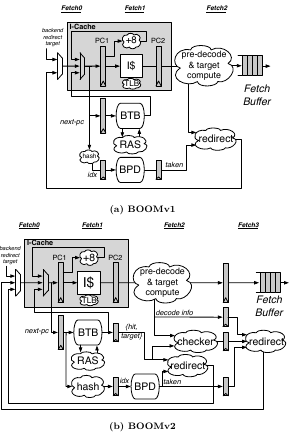
\includegraphics[width=\linewidth]{figs/BOOMbranch.png}
			\captionsetup{labelformat=empty}
			\caption{\small{BOOMv1 and BOOMv2的前端流水线对转图.~\cite{Celio:EECS-2017-157}}}	
			\end{figure}
			
			可以看出v2的转移猜测比v1复杂。而且v2增加了一级并且把BPD的前序工作hash移到F1阶段无非就是消除之前v1的关键路径。同样把BTB改成组相连也是处于消除关键路径的考虑。但是对此新的设计也会因此浪费了一拍即使预测器猜对了,这也是导致IPC下降的原因之一。
			\item \textbf{发射队列(保留站)}
			v1是20 unified entries,而v2则是分为3个队列(integer, memory, floating point),各16 entries.~\cite{Celio:EECS-2017-157}
			\item \textbf{寄存器堆的设计}。我之前并没有注意到会存在这个问题,可是从BOOM的工程实践来看,在v1上,由于采用的是unified的register file,就是无论integer还是FP,都是同一个物理寄存器堆,不仅大,而且读写端口多,造成的后果就是不仅在关键路径上,而且还很难布局布线。所以在v2上,就采用了3种方法去提高register file的性能。\begin{itemize}
				\item 将发射和读寄存器分成两级,issue-select先选出来哪些指令要发射,然后时钟打一拍,下一拍再从寄存器里读取操作数。
				\item 将Integer和FP register分开来。从而降低分别的寄存器的数量以及读写端口的数量。
				\item 最后一个方法是物理的设计,是布局布线的优化,囿于有限的知识水平,就只截了一张图~\cite{Celio:EECS-2017-157}:
				
				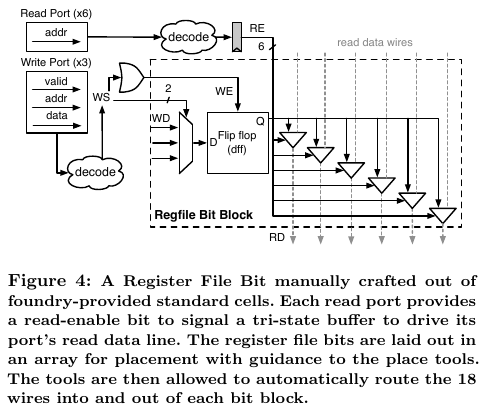
\includegraphics[width=\linewidth]{figs/regfile.png}
			\end{itemize}
			\end{enumerate}
		\end{itemize}
	\end{multicols}

\newpage
\tikz[overlay, remember picture] \draw ([xshift=2.5cm,yshift=-3cm]current page.north west) rectangle ([xshift=-2.5cm,yshift=3cm]current page.south east);
\section*{课题主要研究内容、预期目标:}
	\setcounter{section}{0}
	\section{CPU 设计}
	这一部分是毕业设计中最为核心的部分,由于当前还没有具体的设计,所以只能初步谈谈当前的构思,等到中期报告的时候这一部分会具体展开。但是框架的基础是基于MIPS R10000的。虽然MIPS R10000比Alpha 21264性能低,但是相对而言简单些,同时不难看出BOOM借鉴的更多的也是MIPS R10000。
 	\subsection{instruction fetch}
 	处理器的IPC高不高,首先就要看指令供不供得上,所以这一部分也是优先设计并且测试的模块。本科毕业的设计采用每一排取两条指令的设计。两条指令也即意味着需要两个译码器,译码完成后push到发射队列里面等待发射。
 	\subsubsection{branch prediction}
 	转移猜测是取指器中重中之重的结构。猜测猜什么?猜跳转地址(非直接跳转),猜跳与不跳(分支指令)。几个在BOOM里面提到过的结构BTB,RAS,BPD要实现,同时在Alpha 21264中提到的全局和局部猜测结果混合的技术也可以考虑。现实情况是这一部分很难设计,而且容易成为关键路径。
%The frontend end relies on a number of different branch 	prediction techniques to predict the instruction stream, each trading off accuracy, area, critical path cost, and pipeline penalty when making a prediction.
 	\subsection{multi-issue}
 	指令取回来就要进入发射队列或者叫保留站等待多发射,然后同时进行重命名操作。
 	如果是静态调度的结构,那么指令队列也就是发射队列,但是对于动态调度,保留站在指令队列的下游。一开始的设计从简,所以就先考虑静态的调度。
 	\subsubsection{rename}
 	重命名什么,从逻辑地址到物理地址。所以最多一个目的寄存器需要重命名,最多两个源寄存器地址需要从重命名的表中找到逻辑地址对应的物理地址。
 	\subsection{out-of-order pipeline}
	要多少个ALU,多少个浮点运算器,访存部件队列有多大都是值得商榷的问题,要注意和ROB大小,保留站大小,重命名表大小之间的平衡。
	\subsection{instruction retire \& result commit}
	一次能retire最多几条指令也是要平衡的问题。
 	\subsubsection{precise exception handling}
	例外的硬件处理一定是要做成精确例外的,所以例外的restore state机制要做,必要的信息要加。
 	\subsection{memory system}
 	为了提高性能,除了取指,访存的结构设计也是非常重要的,而且也会复杂。这是因为访存并不是由CPU完全控制的,而且延迟随机。对外接口是握手信号,同时例外处理也要restore访存队列状态,保持到下一次有效访存请求出现。
 	\subsubsection{load \& store mechanism}
	访存队列做多大,outstanding程序要做到什么程度,一拍接受多少个访存请求也是掌握平衡。
 	\subsection{the design which decouples microarchitecture and ISA}
 	由于最后还是要做一个同样微结构的MIPS处理器,所以设计要尽可能的将微结构和ISA解耦合。
 	\section{CPU可同时配置MPIS的generator}
 	不同的ISA怎么比较,我认为最为客观的方法是用一模一样的微结构。而且由于RISC-V和MIPS设计相近,如果完成了一个的设计,切换到另外一个也不是难事。
 	\section{设计空间分析与优化}
	正如前面所说,在具体的设计中有很多有很多的参数大小需要平衡。优化的时候可能还会尝试用到更为复杂的微结构,比如说更为复杂的转移猜测,保留站的模式等等。
	\section{预期目标}
	既然是做多发射乱序的CPU,那么最基本的预期就是性能要比单发射五级静态流水CPU要提高50\%$ \sim $100\%. 同时非常期待RISC-V和MIPS的比较结果。最后更为进阶的目标是能够跑通Linux,甚至能够支持多并且跑多进程能够看到加速比,并奢望能够赶上Cortex A53的水平。也许本科毕设阶段做不完,但这是一个长期的项目。
\newpage
\tikz[overlay, remember picture] \draw ([xshift=2.5cm,yshift=-3cm]current page.north west) rectangle ([xshift=-2.5cm,yshift=3cm]current page.south east);
\section*{拟采用的研究方法、技术路线、实验方案及其可行性分析:}
乱序多发射的CPU是通往高性能处理器的必经之路,Intel、AMD、ARM都应经有了成熟的技术。一个典型的代表就是ARM Cortex A53。作为一个双发射8级静态调度的处理器核,面积很小,功耗很低,SPEC2000 INT base能够达到423分/GHz (\href{https://www.anandtech.com/show/8718/the-samsung-galaxy-note-4-exynos-review/4}{report})
. 但是另外一方面,乱序多发射的设计并不容易,而且比设计更加困难的是调试,如何保证复杂执行的CPU能够有条不紊,毫无错误的运行比如像Linux操作系统这样的大型软件更是难上加难。仅靠一个人的力量是很难在短短数月里面完成的。所幸前有Alpha的技术报告,后有BOOM的开源实现可供参考,而BOOM背后更是有整个RISC-V的开源生态,有整套的调试方法和software stack toolchain。RISC-V作为近些年在总结了前人ISA设计中的利弊的基础上推出的一套设计清晰,干净整洁而优雅的开源ISA,大受学术界工业界的欢迎。鉴于其日臻完善的开源的开发调试工具,有如下考虑方案:
\begin{enumerate}
	\item UC, Berkeley 开发的高级硬件描述语言Chisel对单一时钟,同步复位的电路逻辑的刻画效率比verilog更高,而且对于可综合电路的描述能够做到和verilog同样的精确,故而完全可以采用Chisel进行毕设CPU的设计开发。
	\item 可以参考借鉴开源的BOOM代码实现。
	\item 可以学习借用RISC-V开源调试工具与手段。
	\item 可以低成本地在FPGA平台上的运行目前RISC-V开源的整套以Linux为首的软件栈。
\end{enumerate}

综上,计划的第一步是实现一个基于RISC-V ISA的乱序双发射的CPU,调试完毕能够跑通简单的测试程序,但深知这绝非易事。接着在时间允许的情况下做操作系统的移植,继而能够支持多核。注意到一开始的设计必须考虑到微结构和ISA之间的解耦合,这样将RISC-V改成MIPS工作量会降低很多。得到MIPS版本的CPU目的在于采用相同的微结构可以客观的对比两个ISA的优劣。同时作为工作的非常重要的一部分,性能的优化和设计空间的搜索分析必不可少,会尝试一些方法比如更换各个结构的配置参数,甚至调整逻辑部件的整个结构。

\newpage
\tikz[overlay, remember picture] \draw ([xshift=2.5cm,yshift=-3cm]current page.north west) rectangle ([xshift=-2.5cm,yshift=3cm]current page.south east);
\section*{已有研究基础与所需的研究条件:}
前文的\hyperref[sec:state]{\textbf{\textit{国内外本学科领域的发展现状与趋势}}}已经论述了很多关于已有的研究基础的内容,有代码语言层面的Chisel,有ISA层面的MIPS和主要是RISC-V的设计考虑,有RTL的逻辑设计的前人经验:Alpha 21264, MIPS R10000和BOOM。下来再来论述基于RISC-V的调试方法和software stack以及toolchain.

伯克利分校一开始的RISC-V的开源项目模式是Tethered,而非Standalone Systems模式。这两种模式在本科阶段的实验课都涉及到。大二下的计算机组成原理实验课就是Tethered模式,不能独立运行,要靠其他成熟的Host(如ARM的核)才能运行。大三上的计算机体系结构是Standalone Systems模式,设计的CPU可以独立运行。网上有如何用Rocket的核运行在Xilinx Zynq板卡上并启动运行Linux内核的教程 \url{http://eliaskousk.teamdac.com/entry/welcome}。板卡上用的是ARM A9的核,然后FPGA的配置和组成原理实验课的板卡竟然惊人的相似,所以我就像张科老师要来了一块以前实验课的板卡,准备在以后的几天看看能不能复现。当然复现只是第一步,接下来就是熟悉RISC-V开源的平台,最重要的是调试环境。

首先RISC-V推荐的是他们自行开发的Spike. Spike作为一个软件实现的ISA模拟器,是个ISA interpreter。以tethered RISC-V系统为model,并作为功能正确的基准。设计的目标是快速而且易于修改。对于移植操作系统,RISC-V也有一个Proxy Kernel能够运行在自行设计的CPU上,包括一下特性:\begin{itemize}
	\item 支持单用户进程
	\item I/O相关的系统调用forward到host机上
	\item 实现了Linux ABI的子集
\end{itemize}
而一个完整的Tethered RISC-V Systems还包括Frontend server和Host-Target Interface(HTIF)。Frontend server负责代表proxy kernel执行I/O系统调用。另外一个功能是boot loader(把kernel的ELF文件load到target的memory中)。HTIF是一个host与target的state交互的简单协议。\\
此外RISC-V也有QEMU的Full-System Simulator.\\
而上层的toolchain有Linux,FreeBSD,GCC和LLVM。\\
最后后面要移植到龙芯的MIPS ISA,也有相应的调试环境。\\
具体的调试手段会在中期报告中展开论述。
\newpage
\myFrame{3}{3}
\section*{研究工作计划与进度安排:}
\begin{enumerate}
	\item 2019/01/08$\sim$02/12 把乱序双发射CPU设计完毕。
	\item 2019/02/13$\sim$03/15 一个月后把CPU调试完成,跑通单核的Linux。
	\item 2019/03/16$\sim$03/31 半个月完成移植MIPS的ISA的同样架构的CPU,并调通。
	\item 2019/04/01$\sim$04/15 半个月完成对MPIS和RISC-V的两款CPU进行跑嵌入式benchmark如coremark等程序的量化性能比较与性能分析。
	\item 2019/04/16$\sim$五月中旬 剩下的时间用于性能的调优,量化结果的分析总结,毕业论文的编写。若有余力,考虑多核的架构并能够运行多核的Linux能够有加速比。
\end{enumerate}


\newpage
\myFrame{3}{3}
\bibliographystyle{plain}
\bibliography{mybib}

\includepdf[pages={12},scale=1.15, offset=0mm -10mm]{kaiti.pdf}
\end{document}
